% Ziele: Story hooks
% Mehr Drama als eine Telenovella
% Man muss zig Abenteuer aus der Konstellation ziehen können
% Die Meisten Charaktere sind ü 60 und haben viel erlebt. Das aufzählen.

\chapter{Der Lost Flohmarkt}

Es gibt mehrere Lost Flohmärkte. Dieser hier ist ein mobiler, durch die Lande ziehender Flohmarkt und Treffpunkt verschiedener Lost Gruppen. Doch auch einige Norms und Pioneers werden von diesem angezogen und oft verwirrt zurück gelassen.

Für die Lost ist die Funknachricht, dass bald ein Flohmarkt in ihrer Nähe stattfinden wird, ein wichtiges Ereignis. Doch diesen Flohmarkt zu organisieren bedarf einiges an Aufwand und spezieller Menschen.

Diese speziellen Menschen werden hier vorgestellt.

\section{Wenn alles klappt....}

Wenn diesmal beim Flohmarkt alles klappt ist der Flohmarkt eine bunte Mischung aus Essensdüften, unplugged Musik, Handel und Gefeilsche, Theater, dem Lärm von Schmieden und Tieren. Verschiedenste Dialekte mischen sich. Es ist ist ein großes low tech Festival an dem sich verschiedene sonst verfeindete Gruppen treffen.

Freundschaften werden geschlossen. Pläne geschmiedet und Waren, Geschichten und Gerüchte ausgetauscht.

Nachte beleuchtet von Fackeln und verteilten Lagerfeuern. Gespräche, Gesang und Geschichten bis spät in die Nacht. Es wird getrunken, geraucht und gegessen.

Ca 2 Wochen lange lebt der Ort mit 500 Leuten vor Ort (wobei dauernd An- und Abreisen stattfinden).

Großartige Dinge, die passieren können:

\subsection{Zufallsereignisse}

\begin{enumerate}
    \item Der alte Jacob will sein geheimes Badewannen-Gin Rezept nicht mit ins Grab nehmen. Den ersten drei Personen, die ihm besondere Spirituosen bringen wird er es beibringen.
    \item Nachts gibt es eine spontante Feuerjonglage show
    \item Jemand macht ein Quiz 'Die 1980er Jahre'. zu gewinnen gibt es eine Flasche von Jabobs Badewannen-Gin
    \item Zwei Personen haben sich verlobt. Um das zu feiern kommt eine ganze Sau auf den Grill - das duftet den ganzen Tag über den Flohmarkt. Norms und Pioneers könnten verwirrt reagieren.
    \item Ein Wettstreit findet statt. Zwei Gruppen wollen sich bei Shakespear Darbietungen überbieten. Doch noch fehlen einige passende Personen bei der Besetzung
    \item Erwachsene und Kinder ab 14 können bei der spontant aufgebauten Schießanlage mit halbautomatischen Waffen üben. Norms sind sicher irritiert.
\end{enumerate}


\chapter{Die Aufgabe}

Das Team des Flohmarkts reist durch die Lande, kündigt einen Flohmarkt an, organisiert einen Platz und beginnt diesen herzurichten für um die 500 Personen. Viele der dazukommenden Lost werden zwar selbst beitragen (eigene Essens Stände, Werkstätten).
Doch das Team stellt die Basisinfrastruktur zur Verfügung und versucht verfeindete Gruppen zusammen zu bringen. Denn das ist der Sinn des Flohmarkts (neben Tauschhandel, Wissensaustausch, Unterhaltung).

Die Spielercharaktere treffen auf den Flohmarkt, der gerade aufgebaut wird. Packen an und finden neue Freunde. Nach einigen Tagen ziehen diese weiter, um neue Orte zu bereisen.

\section{Die Probleme}

Beim Aufbau des Lost Flohmarktes kommt es natürlich zu einer Reihe von Problemen. Diese müssen von den NSCs, den Protagonisten und evtl. den neu hinzugekommenen Gäste-Gruppen gelöst werden.

Diese Ortsbeschreibung enthält Erignislisten. Diese haben jeweils 6 Einträge. Falls die Spielleiterin auswürfeln will.

\subsection{Zufallsereignisse beim Aufbau}

\begin{enumerate}
\item Eine Gäste-Gruppe kommt zu spät (Was ist passiert ?)
\item Eine Gäste-Gruppe kommt zu früh (Warum ?)
\item Das Feld auf dem der Flohmarkt stattfinden soll ist nach Starkregen ein See. Mit Brennesseln und Gestrüpp. Der muss zuerst mit schwerem Gerät trocken gelegt werden.
\item Beim Aufbau wird eine verschüttete Lemming Ruine gefunden. Die Jones-es wollen diese durchsuchen. Das kann zu einem Dungeon Crawl führen.
\item Der Aufbau wird verlangsamt, weil die Küche die Leute mit lecker Essen vom Arbeiten abhält
\item Neugierige Kinder aus dem nahen Pioneer Labor kommen mit ihren Exoskeletten zu Besuch - Die Lost reagieren zwischen ängstlich (wegen der Technik) und behütend
\end{enumerate}

\section{Wendy und Familie}

Die NSCs Wendy und ihre Familie wurden so angelegt, dass deren Plotstrang ein Telenovella Level an Drama erzeugt. Wem das nicht in die Stimmung passt, kann diesen Plot gerne modifizieren und runterdimmen.

\chapter{Die Personen}

\section{Tier Experte: Jonas Ohnesorg}

Er organisiert die Unterbringung der Tiere (von Hasen bis zu Rindern). Dabei sorgt er für die Gesundheit der verkauften Tiere und hilft bei der Futterversorgung. Vor-Ort Schlachtungen fallen auch in seine Aufsicht. Eigentlich ist  er Tiertrainer für Raubvögel. Diese reissen aber manchmal Hasen - auch solche in den Freigehegen der Farmer.

\begin{center}
    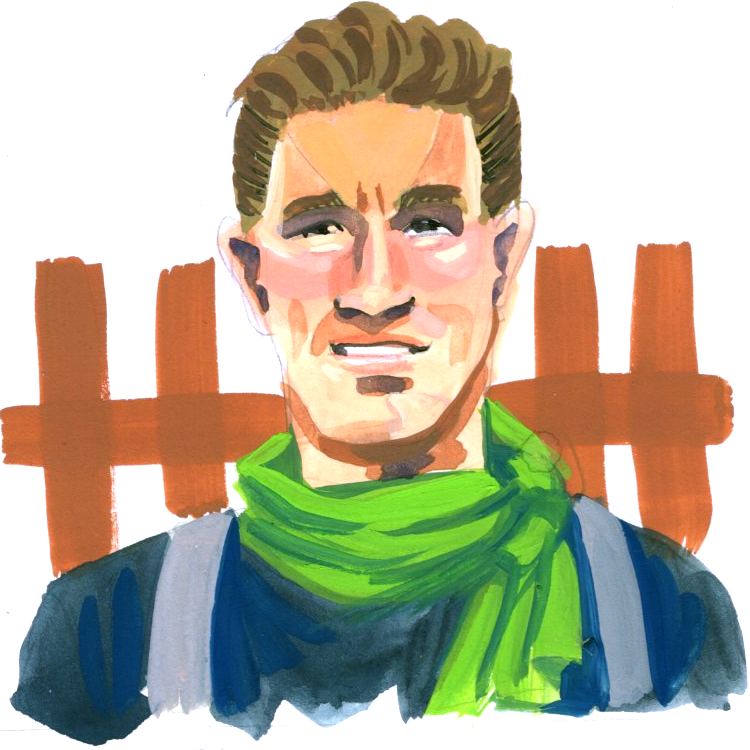
\includegraphics[scale=0.4]{portraits/Flohmarkt_Jonas.png}
\end{center}

\newpage
\begin{npcBox}[title=Jonas Ohnesorg]

    \begin{aspects}
    \item \aspect[Konzept]{Liebt die Tiere mehr als sie ihn lieben}
    \item \aspect[Dilemma]{Irgendwas ermutigt andere immer, seine Tiere unsachgemäß anfassen zu wollen}
    \item \aspect[Beziehung]{Ist in Antigone verliebt}
    \item \aspect[Aspekt]{Isst gerne extrem scharf - er braucht Kicks in seinem Leben}
    \end{aspects}

    \begin{skills}
    \item \nskill{Bildung}{0}
    \item \nskill{Athletik}{1}
    \item \nskill{Diebeskunst}{0}
    \item \nskill{Kontakte}{1}
    \item \nskill{Handwerk}{3}
    \item \nskill{Täuschung}{0}
    \item \nskill{Fahren}{0}
    \item \nskill{Empathie}{1}
    \item \nskill{Kämpfen}{3}
    \item \nskill{Nachforschung}{0}
    \item \nskill{Spezialwissen}{0}
    \item \nskill{Wahrnehmung}{1}
    \item \nskill{Kraft}{2}
    \item \nskill{Provozieren}{0}
    \item \nskill{Charisma}{2}
    \item \nskill{Ressourcen}{0}
    \item \nskill{Schießen}{0}
    \item \nskill{Heimlichkeit}{0}
    \item \nskill{Wille}{2}
    \item \nskill{Bushcraft}{4}
    \end{skills}

    \begin{stunts}
    \item \stunt{Tierflüsterer}{Bekommt +2 auf Bushcraft, um Tiere zu dressieren oder zu befehlen.}
    \end{stunts}

    \begin{stressSection}
    \stressLine{\stress{1}\stress{1}\stress{1}\stress{1}}{\stress{1}\stress{1}\stress{1}\stress{1}}
    \end{stressSection}
    \begin{tabularx}{\textwidth}{ XX }
    \end{tabularx}

    \begin{consequences}
    \item \consequence{2}
    \item \consequence{4}
    \item \consequence{6}
    \end{consequences}

    \begin{equipment}
    \item Igel, sein Adler. Er findet den Namen immer noch lustig
    \item Ausstattung für die verschiedensten Tiere
    \end{equipment}
\end{npcBox}


\subsection{Zufallsereignisse mit Tieren}

\begin{enumerate}
\item Ein Tier bricht aus
\item Ein Tier ist krank - eine Seuchengefahr ? Findet jemand einen (Tier) Arzt ?
\item Trächtige Tiere bekommen ihre Jungen
\item Norms oder Pioneers sind verwirrt von den Tieren. Wollen die streicheln, behalten oder filmen - was schief geht
\item Den Tieren fehlt Futter. Jemand muss schnell richtig viel besorgen
\item Seine Raubvögel reissen anderer Leute Kleintiere
\end{enumerate}

\newpage
\section{Küche und Militärtaktik: Gustav Müller}

Seine Kernthesen: Ordnung, Disziplin und die Saucen sind zentral

Lieblings-doofer Spruch: 'Kein Mampf, kein Kampf'


Zwischen dem Führen einer Küche und einer Schlacht Organisation gibt es kaum Unterschiede'. Für ihn ist beides das Führen kleiner Einheiten. Seine Einstellung bringt ihn zur Verteidigung des Lost Lagers oder zur Großküche für einen Flohmarkt. Mit seiner herrisch militärischen Art kann er zwar Erfolge verbuchen. Doch er macht sich auch Feinde.

Info für SL: So sind Großküchen wirklich entstanden. Aus militärischen Strukturen: \href{https://de.wikipedia.org/wiki/K%C3%BCchenbrigade}{Küchenbrigade}

\begin{center}
    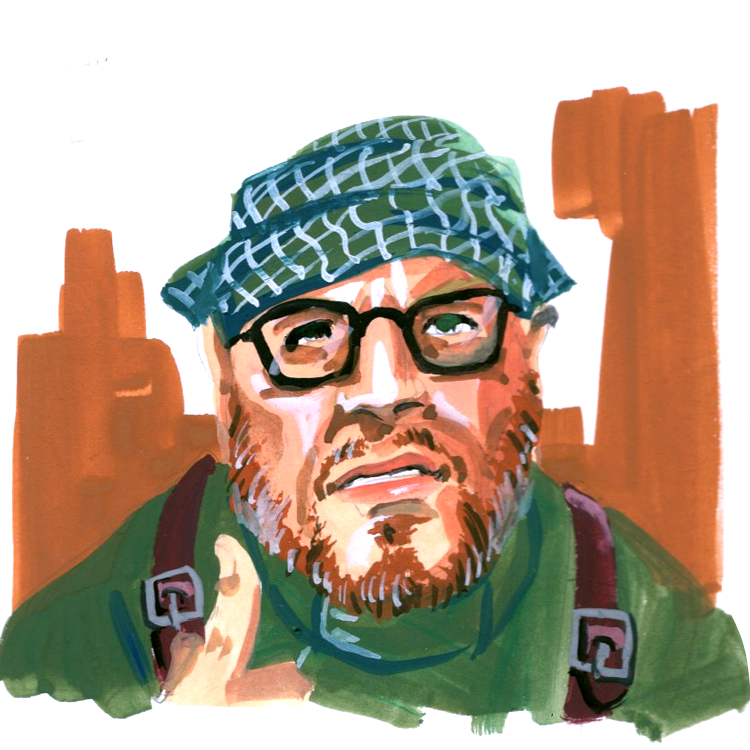
\includegraphics[scale=0.4]{portraits/Flohmarkt_Gustav.png}
\end{center}

\newpage
\begin{npcBox}[title=Gustav Müller]

    \begin{aspects}
    \item \aspect[Konzept]{Perfekt organisierter Küchengeneral}
    \item \aspect[Dilemma]{Hart zu sich selbst - bis zum Umfallen}
    \item \aspect[Beziehung]{Er hat keine engeren Beziehungen zu Menschen}
    \item \aspect[Aspekt]{Die Perfektion erstreckt sich auch in Details - und hübsche Verzierungen}
    \end{aspects}

    \begin{skills}
    \item \nskill{Bildung}{0}
    \item \nskill{Athletik}{1}
    \item \nskill{Diebeskunst}{0}
    \item \nskill{Kontakte}{0}
    \item \nskill{Handwerk - Kochen}{3}
    \item \nskill{Täuschung}{0}
    \item \nskill{Fahren}{1}
    \item \nskill{Empathie}{0}
    \item \nskill{Kämpfen}{1}
    \item \nskill{Nachforschung}{0}
    \item \nskill{Spezialwissen}{2}
    \item \nskill{Wahrnehmung}{1}
    \item \nskill{Kraft}{2}
    \item \nskill{Provozieren}{2}
    \item \nskill{Charisma}{0}
    \item \nskill{Ressourcen}{0}
    \item \nskill{Schießen}{3}
    \item \nskill{Heimlichkeit}{0}
    \item \nskill{Wille}{4}
    \end{skills}

    \begin{stunts}
    \item \stunt{Strukturiert}{Wenn eine klare Hierarchie herrscht, bekommt er +2 auf Handwerk oder Schießen. In chaotischen Hierarchien -2}
    \end{stunts}

    \begin{stressSection}
    \stressLine{\stress{1}\stress{1}\stress{1}\stress{1}}{\stress{1}\stress{1}\stress{1}\stress{1}\stress{1}\stress{1}}
    \end{stressSection}
    \begin{tabularx}{\textwidth}{ XX }
    \end{tabularx}

    \begin{consequences}
    \item \consequence{2}
    \item \consequence{4}
    \item \consequence{6}
    \end{consequences}

    \begin{equipment}
    \item Großkochgeräte. Ganze Anhänger umgebaut zu Küchenelementen
    \item Eine Desert Eagle
    \end{equipment}
\end{npcBox}


\subsection{Zufallsereignisse}

\begin{enumerate}
\item Auf einem LKW ist ein Kräutergarten angelegt. Der steht aber nicht bei den Küchenzelten - weil den jemand vergessen hat. Der muss jetzt irgendwie durch den halb aufgebauten Flohmarkt zur Küche gefahren werden.
\item Man muss aus einem alten Dieselmotor und Getriebe schnell ein riesiges Rührwerk improvisieren
\item Eine lange Tafel wird an einem Tag quer durch den Flohmarkt aufgebaut und alle erhalten ein Festmahl - wenn es denn klappt
\item Gustav überlässt die Küche für ein paar Stunden seinem Sous Chef. Er muss sich um Kampftaktik Übungen im nahen Wald kümmern
\item Er wird gefragt, ob er Schießtraining für Kinder und Erwachsene anbieten kann. Kann er - wenn er Hilfe bei der Küche und der noch zu bauenden Schießanlage bekommt.
\item Leute werden unsaft aus der Küche geworfen. Es gibt Ärger
\end{enumerate}

\newpage

\section{Funk: Antigone Freitag}

Sie kennt jeden aus dem Funk Äther - und kann viele Sprachen. Ihr Ziel ist es, ihre Lemmings-Sammelfiguren komplett zu bekommen: Dazu fragt sie regelmäßig bei ihren Funkkontakten und würde evtl. eine Bergungstrupp losschicken, um eine der fehlenden Figuren zu bergen. Selbst kann sie leider nicht gehen, denn sie sitzt im Rollstuhl. Per Funkgerät kommt aber die gesamte Welt zu ihr.

\begin{center}
    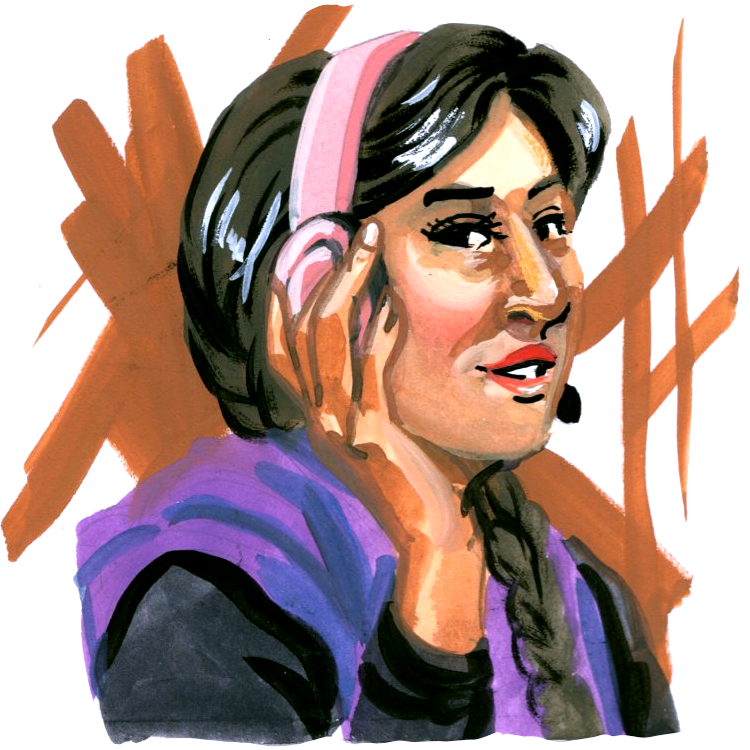
\includegraphics[scale=0.4]{portraits/Flohmarkt_Antigone.png}
\end{center}

\newpage
\begin{npcBox}[title=Antigone]

    \begin{aspects}
    \item \aspect[Konzept]{Funkerin und soziale Enzyklopädie}
    \item \aspect[Dilemma]{Kennt fast jeden eng - hat aber oft keine Ahnung wie Die Leute aussehen}
    \item \aspect[Beziehung]{Dadurch, dass sie jeden sehr gut kennt, hat sie niemanden speziellen}
    \item \aspect[Aspekt]{Mein ausgebildeter kleiner Hund macht mich flexibler und mobiler}
    \end{aspects}

    \begin{skills}
    \item \nskill{Bildung}{3}
    \item \nskill{Athletik}{1}
    \item \nskill{Diebeskunst}{0}
    \item \nskill{Kontakte}{3}
    \item \nskill{Handwerk - Funktechnik}{2}
    \item \nskill{Täuschung}{0}
    \item \nskill{Fahren}{0}
    \item \nskill{Empathie}{2}
    \item \nskill{Kämpfen}{0}
    \item \nskill{Nachforschung}{1}
    \item \nskill{Spezialwissen}{1}
    \item \nskill{Wahrnehmung}{2}
    \item \nskill{Kraft}{0}
    \item \nskill{Provozieren}{0}
    \item \nskill{Charisma}{4}
    \item \nskill{Ressourcen}{0}
    \item \nskill{Schießen}{0}
    \item \nskill{Heimlichkeit}{0}
    \item \nskill{Wille}{1}
    \end{skills}

    \begin{stunts}
    \item \stunt{Mit den Ohren sehen}{Sie ist Funkkontakt so gewöhnt, dass sie mit geschlossenen Augen - nur mit hören - +2 auf Empathie bekommt.}
    \end{stunts}

    \begin{stressSection}
    \stressLine{\stress{1}\stress{1}\stress{1}}{\stress{1}\stress{1}\stress{1}\stress{1}}
    \end{stressSection}
    \begin{tabularx}{\textwidth}{ XX }
    \end{tabularx}

    \begin{consequences}
    \item \consequence{2}
    \item \consequence{4}
    \item \consequence{6}
    \end{consequences}

    \begin{equipment}
    \item Ihr kleiner Mischlingshund 'Snack', der ihr auf Befehl Dinge bringen kann
    \item Funkgeräte
    \item Lötstation
    \end{equipment}
\end{npcBox}

\subsection{Zufallsereignisse}

\begin{enumerate}
\item Sie hat jemanden per Funk gefunden, der Sammelfiguren hat. Und die Person ist auf dem Flohmarkt. Da kein Funkkontakt besteht, müssen die Protagonisten die Person per Beschreibung finden
\item Eine anreisende Truppe ist in Gefahr und die PC müssen sie her leiten
\item Funkrepeater müssen gebaut und an Gruppen verteilt werden, die bald abreisen
Das Funkgerät fällt aus. Schnell wird ein Verstärker und Elektronik vom Flohmarkt benötigt
\item Sie will den Flohmarkt auch mal durchreisen. Nur ist der Rollstuhl unpraktisch im Schlamm. Sie braucht Hilfe. Bei der Reise wird sie viele der Leute zum ersten mal sehen, mit denen sie sonst nur redet.
\item Sie will ein Flohmarkt-Radioprogramm senden. Empfänger müssen verteilt werden und Inhalt erstellt.
\end{enumerate}

\newpage

\section{Gaia Priester Laura}

Laura, Gaianistin. Sie ist eine unerfahrene Priesterin, in einer sich selbst gerade gründenden Religion. Da sie abgeschieden ist, ist sie für jeden spirituellen Input (Bücher, Gespräche) sehr dankbar. Oft versucht sie auch, anderen Gaia zu erklären - stolpert dabei aber schnell, sobald es komplexer wird.

\begin{center}
    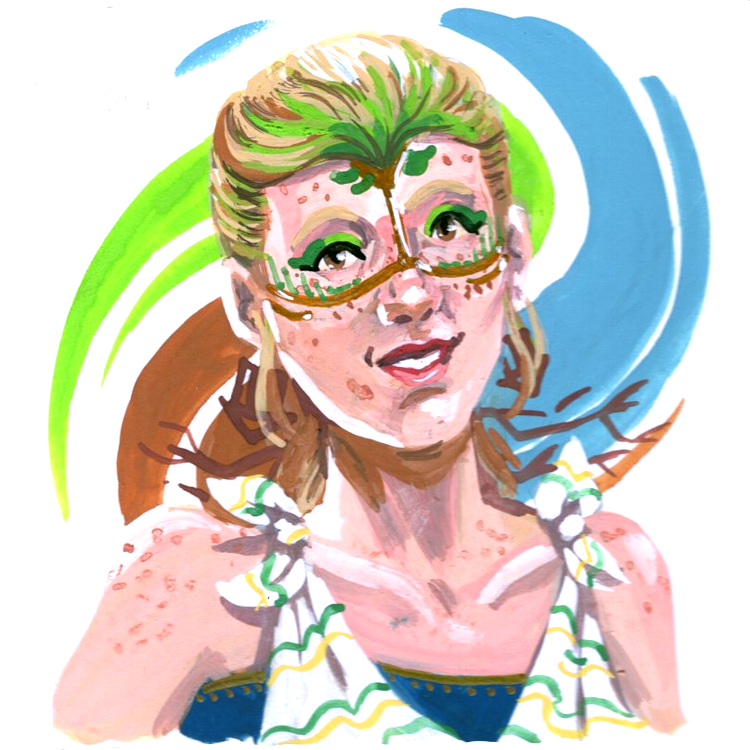
\includegraphics[scale=0.4]{portraits/Flohmarkt_Laura.png}
\end{center}

\newpage
\begin{npcBox}[title=Laura, Gaianistin]

    \begin{aspects}
    \item \aspect[Konzept]{Beginnende Gaianistin}
    \item \aspect[Dilemma]{Die Schuhe sind zu groß}
    \item \aspect[Beziehung]{Sie hat sich frisch der Flohmarkt Gruppe angeschlossen und kennt noch niemanden}
    \item \aspect[Aspekt]{Frisch den Weg gefunden, hoch begeistert und noch stolpernd}
    \end{aspects}

    \begin{skills}
    \item \nskill{Bildung}{3}
    \item \nskill{Athletik}{1}
    \item \nskill{Diebeskunst}{0}
    \item \nskill{Kontakte}{1}
    \item \nskill{Handwerk}{0}
    \item \nskill{Täuschung}{0}
    \item \nskill{Fahren}{0}
    \item \nskill{Empathie}{3}
    \item \nskill{Kämpfen}{0}
    \item \nskill{Nachforschung}{2}
    \item \nskill{Spezialwissen}{2}
    \item \nskill{Wahrnehmung}{1}
    \item \nskill{Kraft}{0}
    \item \nskill{Provozieren}{0}
    \item \nskill{Charisma}{4}
    \item \nskill{Ressourcen}{1}
    \item \nskill{Schießen}{0}
    \item \nskill{Heimlichkeit}{0}
    \item \nskill{Wille}{2}
    \end{skills}

    \begin{stunts}
    \item \stunt{Mandala}{Mit den richtigen Materialien und Zeit kann sie ein inspirierendes Mandala legen, das aufmerksamen Betrachtern +2 auf Wille gibt. Das Mandala hält selbst mit Pflege max. 2 Tage}
    \end{stunts}

    \begin{stressSection}
    \stressLine{\stress{1}\stress{1}\stress{1}}{\stress{1}\stress{1}\stress{1}\stress{1}}
    \end{stressSection}
    \begin{tabularx}{\textwidth}{ XX }
    \end{tabularx}

    \begin{consequences}
    \item \consequence{2}
    \item \consequence{4}
    \item \consequence{6}
    \end{consequences}

    \begin{equipment}
    \item Teekräuter - frisch und getrocknet
    \item Teezelt
    \end{equipment}
\end{npcBox}


Gaia Priester haben sich der lebendigen Erde - Gaia verschrieben. Der Einheit der Öko/Techno und Soziosphäre. Sie versuchen besonders, andere Leute zu animieren, Brücken zu bauen. Brücken zwischen verfeindeten Gruppen z.B. und dabei gemeinsam Projekte umzusetzen.

\newpage


\section{Heavy machines: Wendy}

Chef Logistikerin, Heavy machines und Truckerin: Wendy (früher Wilhelm). Ihre Ehe mit Doris hat sich vor der Katastrophe zerrüttet. Sie wusste auch nicht warum. Später hat sie festgestellt, dass sie Trans und damit eine Frau ist. Sie hat ein Foto aus der Alten Zeit hinter der Sonnenblende. Er zusammen mit Doris, seiner Frau. Sie waren vor den Katastrophen mit dem Truck durch Europa unterwegs. Die Ehe scheiterte, weil Wilhelm/Wendy immer unterwegs war und Doris eher sesshaft. Aus der Ehe stammt ein Kind, 'Flash'. Dass Wendy mal Wilhelm war, wissen die Lost nicht.

\begin{center}
    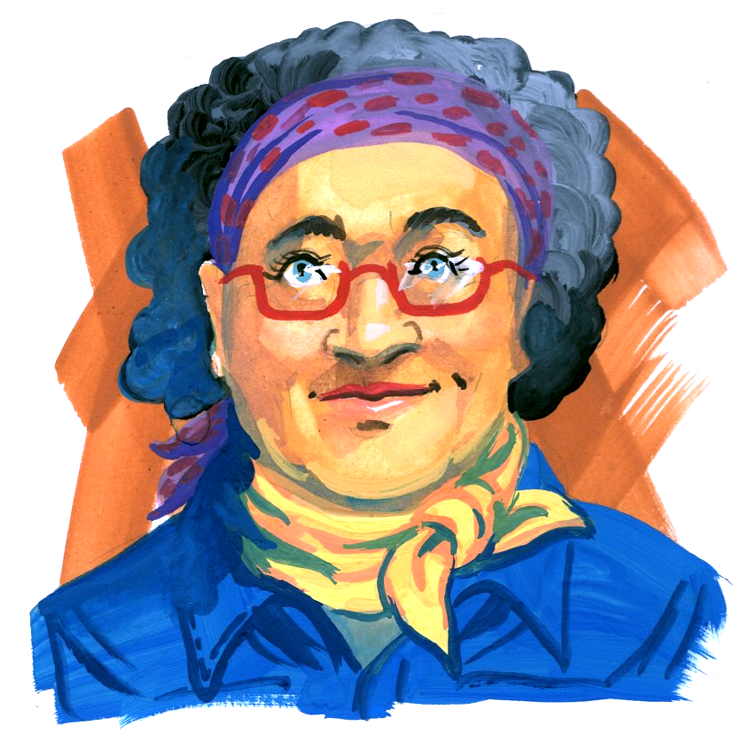
\includegraphics[scale=0.4]{portraits/Flohmarkt_Wendy.png}
\end{center}

\newpage
\begin{npcBox}[title=Wendy]

    \begin{aspects}
    \item \aspect[Konzept]{Große Maschinen machen mich glücklich}
    \item \aspect[Dilemma]{Auf der Straße zuhause}
    \item \aspect[Beziehung]{Gescheiterte Ehe mit Doris, weil Doris zu sesshaft ist.}
    \item \aspect[Aspekt]{Tägliches Training ist nötig für meine Psyche}
    \end{aspects}

    \begin{skills}
    \item \nskill{Bildung}{0}
    \item \nskill{Athletik}{1}
    \item \nskill{Diebeskunst}{0}
    \item \nskill{Kontakte}{0}
    \item \nskill{Handwerk}{3}
    \item \nskill{Täuschung}{0}
    \item \nskill{Fahren}{4}
    \item \nskill{Empathie}{2}
    \item \nskill{Kämpfen}{0}
    \item \nskill{Nachforschung}{0}
    \item \nskill{Spezialwissen}{0}
    \item \nskill{Wahrnehmung}{2}
    \item \nskill{Kraft}{3}
    \item \nskill{Provozieren}{1}
    \item \nskill{Charisma}{1}
    \item \nskill{Ressourcen}{0}
    \item \nskill{Schießen}{0}
    \item \nskill{Heimlichkeit}{0}
    \item \nskill{Wille}{2}
    \item \nskill{Bushcraft}{1}
    \end{skills}

    \begin{stunts}
    \item \stunt{Schwergewicht}{Wendy bekommt +2 auf Fahren, wenn das Fahrzeug mehr als 5 Tonnen wiegt.}
    \end{stunts}

    \begin{stressSection}
    \stressLine{\stress{1}\stress{1}\stress{1}\stress{1}\stress{1}\stress{1}}{\stress{1}\stress{1}\stress{1}\stress{1}}
    \end{stressSection}
    \begin{tabularx}{\textwidth}{ XX }
    \end{tabularx}

    \begin{consequences}
    \item \consequence{2}
    \item \consequence{4}
    \item \consequence{6}
    \end{consequences}

    \begin{equipment}
    \item Zugriff auf Bagger, Lastwagen und Stapler der Flohmarkt Organisation
    \item Ein Satz Gewichte fürs Training
    \item Schminkset
    \end{equipment}
\end{npcBox}
\newpage

\section{Norm Dokumentatorin Doris}

Sie ist auf Abenteuer Trip (ohne Sanitäre Einrichtung und ohne Kunstfleisch, Drohnen oder Vernetzung): War früher mit Wilhelm verheiratet. Trägt immer noch den Ring in ihrer Tasche, weiss aber nicht, dass es Wendy ist. Kommen sie wieder zusammen ?
Den Abenteuer Trip unternimmt sie, weil sie mit Freunden gewettet hat. Die Freunde wissen, dass ihr Ex dort irgendwo unter den Lost ist und hoffen, die kommen wieder zusammen. Denn ihnen hat Doris oft von der gemeinsamen Zeit erzählt.

\begin{center}
    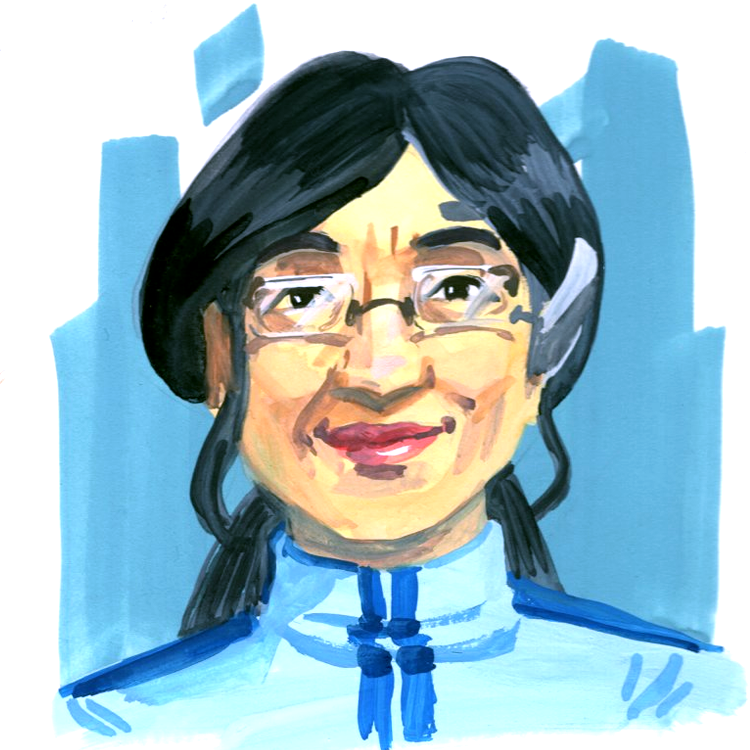
\includegraphics[scale=0.4]{portraits/Flohmarkt_Doris.png}
\end{center}

\newpage
\begin{npcBox}[title=Doris]

    \begin{aspects}
    \item \aspect[Konzept]{Stadtverwöhnt und auf Abenteuer}
    \item \aspect[Dilemma]{Auf der Suche nach verlorener Vergangenheit}
    \item \aspect[Beziehung]{Ihre Freund wissen besser als sie, wer ihr fehlt}
    \item \aspect[Aspekt]{Sesshaft - mit starken Verbindungen}
    \end{aspects}

    \begin{skills}
    \item \nskill{Bildung}{3}
    \item \nskill{Athletik}{0}
    \item \nskill{Diebeskunst}{0}
    \item \nskill{Kontakte}{1}
    \item \nskill{Handwerk}{0}
    \item \nskill{Täuschung}{0}
    \item \nskill{Fahren}{0}
    \item \nskill{Empathie}{3}
    \item \nskill{Kämpfen}{0}
    \item \nskill{Nachforschung}{1}
    \item \nskill{Spezialwissen}{0}
    \item \nskill{Wahrnehmung}{2}
    \item \nskill{Kraft}{0}
    \item \nskill{Provozieren}{0}
    \item \nskill{Charisma}{4}
    \item \nskill{Ressourcen}{2}
    \item \nskill{Schießen}{0}
    \item \nskill{Heimlichkeit}{1}
    \item \nskill{Wille}{1}
    \item \nskill{Hive Kontrolle}{2}
    \end{skills}

    \begin{stunts}
    \item \stunt{Den Wald sehen}{In fremder Umgebung ist sie besonders aufmerksam. Wenn sie Lost oder Pioneer Eigenheiten beobachtet, bekommt sie +2 auf Wahrnehmung.}
    \end{stunts}

    \begin{stressSection}
    \stressLine{\stress{1}\stress{1}\stress{1}}{\stress{1}\stress{1}\stress{1}\stress{1}}
    \end{stressSection}
    \begin{tabularx}{\textwidth}{ XX }
    \end{tabularx}

    \begin{consequences}
    \item \consequence{2}
    \item \consequence{4}
    \item \consequence{6}
    \end{consequences}

    \begin{equipment}
    \item Ihren Hive Controller
    \item Einen Hive Funk Repeater, der nur manchmal funktioniert. Kaputt ? Sollte er tun kann sie Dinge aus dem Hive per Drohne bestellen
    \end{equipment}
\end{npcBox}
\newpage

\section{Pioneer Tochter 'Flash'}

Die Tochter von Doris und Wilhelm/Wendy. Ca. 35 Jahre alt. Sie ist sehr aktiv und unstet. Flash ist mit ihrer Mutter leicht zerstritten (wegen ihr kein Kontakt zum Vater, und die Mutter ist eine langweilige Norm). Weiss aber, dass der Vater Wendy heisst und bei den Lost ist, Leider hat sie keine Ahnung, wie sie sich ihm vorstellen soll. Für sie ist eine originelle Geschlechtsidentität absolut üblich.

\begin{center}
    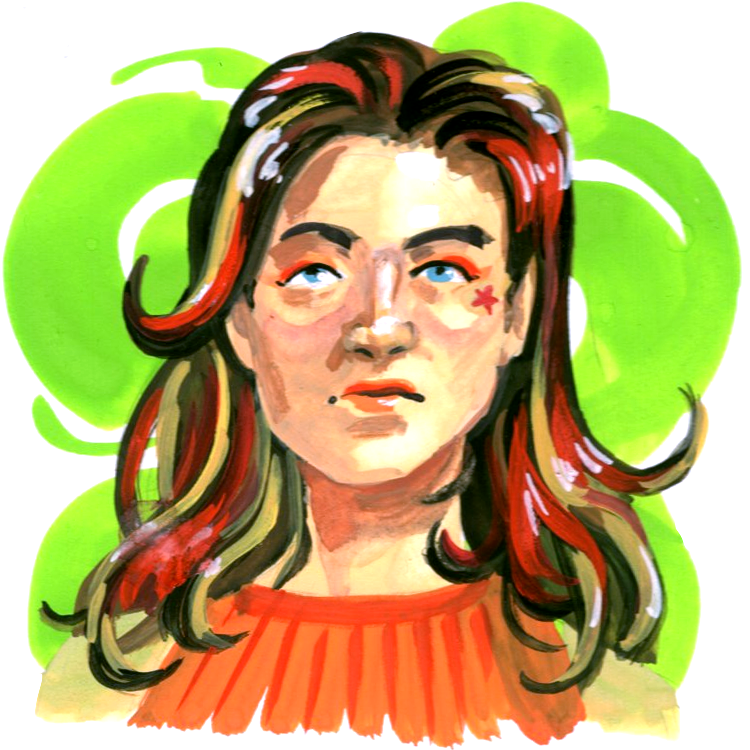
\includegraphics[scale=0.4]{portraits/Flohmarkt_Flash.png}
\end{center}

\newpage
\begin{npcBox}[title=Flash]

    \begin{aspects}
    \item \aspect[Konzept]{Zukunfts gestaltende Genetik Expertin}
    \item \aspect[Dilemma]{Zerstritten mit der Familie, die sie liebt}
    \item \aspect[Beziehung]{Sie findet es normaler, eine Frau als Vater zu haben, als diese selbst}
    \item \aspect[Aspekt]{E-Bike süchtig}
    \end{aspects}

    \begin{skills}
    \item \nskill{Bildung}{3}
    \item \nskill{Athletik}{1}
    \item \nskill{Diebeskunst}{0}
    \item \nskill{Kontakte}{0}
    \item \nskill{Handwerk}{3}
    \item \nskill{Täuschung}{1}
    \item \nskill{Fahren}{1}
    \item \nskill{Empathie}{0}
    \item \nskill{Kämpfen}{0}
    \item \nskill{Nachforschung}{2}
    \item \nskill{Spezialwissen}{2}
    \item \nskill{Wahrnehmung}{0}
    \item \nskill{Kraft}{0}
    \item \nskill{Provozieren}{0}
    \item \nskill{Charisma}{1}
    \item \nskill{Ressourcen}{0}
    \item \nskill{Schießen}{0}
    \item \nskill{Heimlichkeit}{0}
    \item \nskill{Wille}{2}
    \item \nskill{Prototyping}{4}
    \end{skills}

    \begin{stunts}
    \item \stunt{Kleinvieh}{Bevorzugt kleine und wendige Fahrzeuge. Bei allen Fahrzeugen, die leichter sind als sie, bekommt sie +2 auf Fahren.}
    \end{stunts}

    \begin{stressSection}
    \stressLine{\stress{1}\stress{1}\stress{1}}{\stress{1}\stress{1}\stress{1}\stress{1}}
    \end{stressSection}
    \begin{tabularx}{\textwidth}{ XX }
    \end{tabularx}

    \begin{consequences}
    \item \consequence{2}
    \item \consequence{4}
    \item \consequence{6}
    \end{consequences}

    \begin{equipment}
    \item Ein E-Bike dass jenseits aller Vernunft getuned ist
    \item Ein Gentech Kit, mit dem man Diagnosen machen kann und einfachste Eingriffe
    \end{equipment}
\end{npcBox}
\newpage

\chapter{Andere Gruppen}

Lost Flohmärkte wollen gezielt mehrere Lost Gruppen zusammen bringen. Doch oft findet man auch leicht verwirrte Pioneers und Norms.

\section{Jones-es}

So nennt sich eine Gruppe, die in den Ruinen der Lemminge nach Technologie, Büchern und anderen wertvollen oder interessante Dingen sucht. Sie bieten ihre letzten Funde an. Dafür benötigen sie Medikamente und Reperaturen.

\subsection{Zufallsfunde aus den Ruinen}

\begin{enumerate}
    \item Eine Kiste alter und gut erhaltener Weinflaschen. Und viele Dosenravioli.
    \item Perry Rhodan Silberbände
    \item Private Video Kasetten aus den 1990er - was da wohl drauf ist ?
    \item Eine alte Landkarte dieser Region. Doch viele der Orte sind nach den Katastrophen nicht mehr vorhanden. Lohnt sich eine Expedition ?
    \item Ein Kinder-Aufsatz 'So stelle ich mir die Zukunft vor'. Was da wohl drin steht ? Was aus dem Kind geworden ist ?
    \item Eine Kiste voller alter Brettspiele
\end{enumerate}

Am wertvollsten sind die Artefakte aus der alten Welt, die die Lost bei Expeditionen geborgen haben. Die Artefakte der Lemminge. Insbesondere die Lost sind auf alte Technologie angewiesen, um ihre Fahrzeuge und Gebäude zu reparieren. Bücher selbst haben aber einen fast spirituellen Wert für die Lost und seltene Exemplare würden auf dem Flohmarkt heimlich gehandelt. Bis sie jemand um Ruhm zu ernten nach 'Alexandria' bringt, wo sie kopiert und vervielfältigt werden.

Lost handeln übrigens im Tauschhandel, Norms bezahlen mit digitalem Geld und bei Pioneers finden viele Transaktionen eher über Ruf und Ruhm der Personen statt. Auf einem Lost Flohmarkt sind also gerade für nicht-Lost Kulturschocks und chaotische Ketten an Tauschhandel vorprogrammiert.

\section{Farmer}

Suchen Tiere zur Zucht und Pflanzensamen. Sie sind bereit mit Naturalien zu zahlen. Spontane Schlachtungen für den Festbraten sind auch zu erwarten. Die vielen Tiere können ein Mist-Entsorgungs Problem verursachen und massiven Gestank, wenn man das nicht im Vorfeld einplant.

\section{Handwerker}

Sie bieten Reperaturen, benötigen aber Rohstoffe.

\section{Der Jahrmarkt}

Natürlich gibt es noch hunderte Lost aus andere Gruppen, die kochen, reparieren, verkaufen, kaufen, vorlesen, musizieren, suchen und einen Jahrmarkt betreiben mit aller Art von Buden und Attraktionen. Bei Kinder beliebt: Wetten auf eine Maus in einem Labyrinth: Welchen Ausgang wird sie nehmen ?


